\subsection{Red-Black Trees}

\begin{frame}{Red-Black-Trees}{Introduction}
  \textbf{Red-Black Tree:}
  \begin{itemize}
    \item
      Binary tree with {\color{Mittel-Blau}red} and {\color{Mittel-Blau}black}
      nodes
    \item
      Number of {\color{Mittel-Blau}black} nodes on path to leaves is  equal
    \item
      Can be interpreted as {\color{Mittel-Blau}(2,4)-tree}
      (also named 2-3-4-tree)
    \item
      Each {\color{Mittel-Blau}(2,4)-tree}-node is a small red-black-tree
      with a {\color{Mittel-Blau}black} root node
  \end{itemize}
\end{frame}

%-------------------------------------------------------------------------------

\begin{frame}{Red-Black-Trees}{Introduction}
  \begin{figure}
    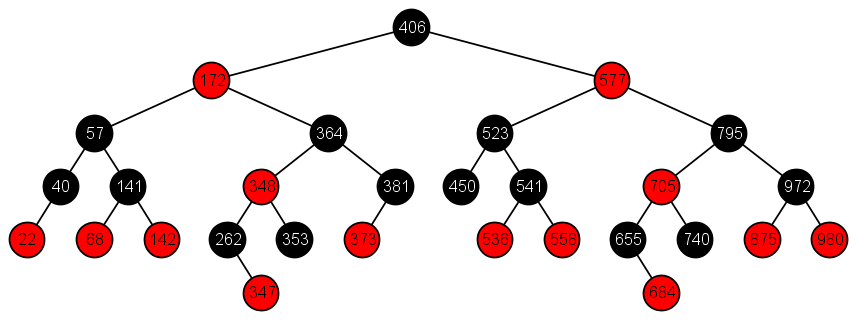
\includegraphics[width=\textwidth]
      {Lecture/Images/Red-Black-Tree/Red-Black-Tree.png}
    \caption{Example of an
      {\color{Mittel-Blau}red-black-tree}~\cite{gnarley_trees}}
    \label{fig:red_black_tree:red_black_tree_introduction}
  \end{figure}
\end{frame}
